% Author: Izaak Neutelings (July 2018)
% page 8 https://archive.org/details/StaticAndDynamicElectricity
% https://tex.stackexchange.com/questions/56353/extract-x-y-coordinate-of-an-arbitrary-point-on-curve-in-tikz
% https://tex.stackexchange.com/questions/412899/tikz-calculate-and-store-the-euclidian-distance-between-two-coordinates
\documentclass[border=3pt,tikz]{standalone}
\usepackage{amsmath} % for \dfrac
\usepackage{bm}
\usepackage{physics}
\usepackage{tikz,pgfplots}
\usetikzlibrary{angles,quotes} % for pic (angle labels)
\usetikzlibrary{calc}
\usetikzlibrary{decorations.markings}
\tikzset{>=latex} % for LaTeX arrow head

\usepackage{xcolor}
\colorlet{Ecol}{orange!90!black}
\colorlet{EcolFL}{orange!80!black}
\colorlet{veccol}{green!45!black}
\colorlet{EFcol}{red!60!black}
\tikzstyle{charged}=[top color=blue!20,bottom color=blue!40,shading angle=10]
\tikzstyle{darkcharged}=[very thin,top color=blue!60,bottom color=blue!80,shading angle=10]
\tikzstyle{redcharged}=[very thin,top color=red!60,bottom color=red!80,shading angle=10]
\tikzstyle{charge+}=[very thin,top color=red!80,bottom color=red!80!black,shading angle=-5]
\tikzstyle{charge-}=[very thin,top color=blue!50,bottom color=blue!70!white!90!black,shading angle=10]
\tikzstyle{gauss surf}=[green!40!black,top color=green!2,bottom color=green!80!black!70,shading angle=5,fill opacity=0.5]
\tikzstyle{gauss lid}=[gauss surf,middle color=green!80!black!20,shading angle=40,fill opacity=0.6]
\tikzstyle{gauss dark}=[green!50!black,fill=green!60!black!70,fill opacity=0.8]
\tikzstyle{gauss line}=[green!40!black]
\tikzstyle{gauss dashed line}=[green!60!black!80,dashed,line width=0.2]
\tikzstyle{EField}=[->,thick,Ecol]
\tikzstyle{vector}=[->,thick,veccol]
\tikzstyle{normalvec}=[->,thick,blue!80!black!80]
\tikzstyle{EFieldLine}=[thick,EcolFL,decoration={markings,
          mark=at position 0.5 with {\arrow{latex}}},
          postaction={decorate}]
\tikzstyle{measure}=[fill=white,midway,outer sep=2]
\def\L{8}
\def\W{0.25}
\def\N{14}


\begin{document}



% ROD ELECTRIC FIELD VERTICAL
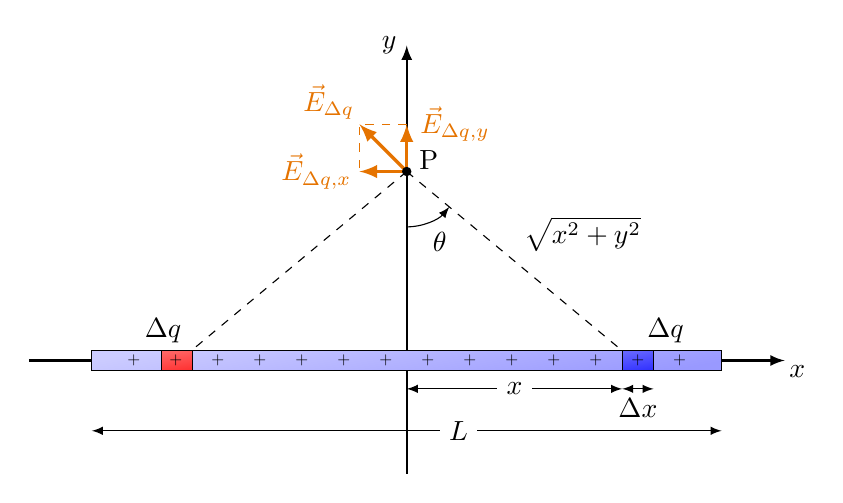
\begin{tikzpicture}
  
  \def\xmax{0.6*\L}
  \def\ymin{-0.18*\L}
  \def\ymax{0.5*\L}
  \def\x{0.342*\L}
  \def\lx{0.390*\L}
  \def\dx{0.05*\L}
  \coordinate (O) at (0,0);
  \coordinate (P) at (0,{0.6*\ymax});
  \coordinate (X) at (\x,\W/2);
  \coordinate (A) at (-\x,\W/2);
  
  % AXIS
  \draw[->,thick] (-\xmax,0) -- (\xmax,0) node[below right=-2] {$x$};
  \draw[->,thick] (0,\ymin) -- (0,\ymax) node[left] {$y$};
  
  % MEASURES
  %\draw[<->] (0,0.2*\ymax) --++ (\x,0) node[midway,above] {$x$};
  \draw[<->] (    0,0.25*\ymin) --++ (\x,0) node[measure] {$x$};
  \draw[<->] (   \x,0.25*\ymin) --++ (\dx,0) node[midway,below] {$\Delta x$};
  \draw[<->] (-\L/2,0.62*\ymin) --++ (\L,0) node[measure,right=10] {$L$};
  
  % VECTORS
  \draw[EField,very thick] (P) --++ ( 0.0,0.6) node[right=1] {${\vec{E}_{\Delta q, y}}$};
  \draw[EField,very thick] (P) --++ (-0.6,0.0) node[left=-1] {${\vec{E}_{\Delta q, x}}$};
  \draw[EField,very thick] (P) --++ (-0.6,0.6) node[above left=-2] {$\vec{E}_{\Delta q}$};
  \draw[EField,-,dashed,thin] (P) ++ (0,0.6) --++ (-0.6,0) --++ (0,-0.6);
  
  % POINT
  \fill (P) circle (0.06) node[above=4,right=1] {P};
  \draw[dashed] (P) -- (X) node[midway,above right] {$\sqrt{x^2+y^2}$};
  \draw[dashed] (P) -- (A);
  \draw pic[->,"$\theta$",draw=black,angle radius=20,angle eccentricity=1.4] {angle = O--P--X};
  %\draw[vector] (X) -- ($(X)!0.12!(P)$) node[right=5,above=-2] {$\vu{r}$};
  
  % ROD
  \draw[charged] (-\L/2,-\W/2) rectangle ++(\L,\W);
  \draw[darkcharged] (\x,-\W/2) rectangle ++(\dx,\W)
    node[midway,right=10,above=3] {$\Delta q$};
  \draw[redcharged] (-\lx,-\W/2) rectangle ++(\dx,\W)
    node[midway,left=5,above=3] {$\Delta q$};
  \foreach \i [evaluate={\x=-\L/2+\i*\L/(\N+1);}] in {1,...,\N}{
    \node[scale=0.6] at (\x,0) {$+$};
  }
  
\end{tikzpicture}

\end{document}